\documentclass[12pt]{article}

\usepackage[T1]{fontenc}
\usepackage[utf8]{inputenc}
\usepackage{mathptmx}
\usepackage{microtype}
\usepackage[a4paper,margin=1in]{geometry}
\usepackage{amsmath}
\usepackage{amssymb}
\usepackage{graphicx}
\usepackage{enumitem}
\usepackage{titlesec}
\usepackage{tabularx}
\usepackage{booktabs}
\usepackage{ragged2e}
\usepackage{xcolor}
\usepackage{hyperref}
\usepackage{natbib}
\bibliographystyle{plainnat}

\definecolor{accent}{HTML}{1F4E79}

\hypersetup{
  colorlinks=true,
  linkcolor=accent,
  urlcolor=accent,
  citecolor=accent
}

\titleformat{\section}{\Large\bfseries\color{accent}}{\thesection.}{0.5em}{}
\titleformat{\subsection}{\large\bfseries\color{accent}}{\thesubsection}{0.5em}{}
\titleformat{\subsubsection}{\normalsize\bfseries\itshape\color{accent}}{\thesubsubsection}{0.5em}{}

\linespread{1.0}
\setlength{\parskip}{0pt}
\setlength{\parindent}{1em}
\setlength{\emergencystretch}{2em}

\begin{document}

%% Title page
\begin{titlepage}
\centering
\vspace*{0.2cm}

{\LARGE\bfseries\color{accent} Performative Prediction\\ in a Single-Asset Market\par}
\vspace{0.5em}
{\large\itshape Self-Fulfilment, Signal Erosion, and Economic\\ Value under Forecast Adoption\par}

\vspace{0.9cm}


\includegraphics[width=0.30\textwidth]{IELogo.jpeg}

\vspace{0.9cm}

{\Large Jan Jacek Wejchert\par}
\vspace{0.3em}
{\large June 2026\par}

\vspace{0.8cm}
\rule{0.7\textwidth}{0.4pt}\par
\vspace{0.4em}

{\Large\bfseries\color{accent} Abstract\par}
\vspace{0.3em}

\begin{minipage}{0.86\textwidth}
\justifying\small
This report studies how widespread adoption of a shared autoregressive forecasting rule affects forecast performance and economic value in a single-asset agent-based market. The market combines Brock-Hommes mean-variance demand with a Beja-Goldman / Farmer-Joshi market-maker price update. Traders may switch from a no-skill null rule to a public rolling AR forecast under either exogenous stochastic diffusion or endogenous certainty-equivalent switching. The forecast is evaluated against two distinct targets on the same path: the realised return, which is the metric a deployed forecaster actually sees, and a demand-adjusted counterfactual that strips out contemporaneous price impact.

The simulator identifies a dual-channel result. As adoption rises, the rolling out-of-sample $R^{2}$ against realised returns reaches roughly 0.19 at full adoption, against 0.07 for a zero-adoption control on the same shocks, through coordinated adopter demand. The same forecast's $R^{2}$ against the demand-adjusted return falls to roughly 0.04, against 0.08 under the control, with the rolling effective AR coefficient rising from 0.28 to 0.45 in step. Mean adopter profit is amplified rather than eroded in the cost-free baseline; the null-relative economic comparison is dominated by position-size asymmetry between the null rule and the capped adopter rule and is reported with that caveat. The headline summary is therefore that adoption raises realised predictive performance through a self-fulfilment channel while reducing the independent demand-adjusted signal the forecast was originally designed to exploit.
\end{minipage}

\vfill
\end{titlepage}

\tableofcontents
\newpage


\section{Introduction}

\subsection{Motivation}

\subsection{Relation to previous work}

\subsection{Research question and contribution}

\subsection{Report roadmap}


\section{Background and theoretical framework}

\subsection{Reflexivity and performative prediction}

\subsection{Heterogeneous-agent finance and price formation}

\subsection{Forecast evaluation under self-fulfilment}

\subsection{Key concepts and notation}


\section{The model}

\subsection{Single-asset market with linear price impact}

\subsection{Trader behaviour: belief, decision, and switching layers}

\subsection{Null rule and rolling AR forecasting rule}

\subsection{Adoption mechanisms}

\subsubsection{Stochastic diffusion}

\subsubsection{Certainty-equivalent performance-based switching}

\subsection{Intra-period timing}

\subsection{The realised vs demand-adjusted decomposition}


\section{Metrics and experimental design}

\subsection{Primary forecast-performance endpoints}

\subsubsection{Realised-return $R^{2}$}

\subsubsection{Demand-adjusted-return $R^{2}$}

\subsection{Primary economic endpoint}

\subsection{Effective AR coefficient as a market-dynamics diagnostic}

\subsection{Target-specific critical adoption shares}

\subsection{Simulation protocol, seed handling, and parameter grid}


\section{Implementation}

\subsection{Software architecture}

\subsection{Phased construction}

\subsection{Reproducibility}


\section{Results}

\subsection{Baseline market and benchmark validation (phases 1 and 2)}

Phase 1 checks that the simulator reproduces the baseline market of section 3.1 of the proposal when every trader follows the random null rule of section 3.3. A single run uses $N=200$ traders, $T=5000$ periods, price-impact coefficient $\mu=0.05$, input autoregressive coefficient $\varphi=0.10$ in the return law $r_{t+1}=\varphi r_t+\mu D_t+\sigma\varepsilon_{t+1}$, news scale $\sigma=0.01$, null-order scale $\sigma_q=1.0$, and seed 42. % src: notebooks/phase_01_baseline_market.ipynb parameters cell (cell 1); phase_01_baseline.npz['seed']
Null orders are independent Gaussian draws, so aggregate demand $D_t$ is directionally uninformative and feeds the return only as unpredictable price-impact noise; the only structure in returns that a forecast could exploit is the $\varphi r_t$ term. The run behaves accordingly. The log price wanders without systematic drift (the mean one-step return of $2.0\times10^{-4}$ sits within 1.4 standard errors of zero), and the return series is roughly stationary with standard deviation $0.0105$. % src: phase_01_baseline.npz['returns'] (mean = 1.998e-4, std = 0.01050, se = std/sqrt(5000) = 1.485e-4); results/figures/phase_01_price_path.png
The empirical lag-1 autocorrelation of returns is $0.103$, matching the input $\varphi=0.10$ within the sampling error of roughly $1/\sqrt{T}\approx0.014$ for a series of this length. % src: phase_01_baseline.npz['phi_empirical'] vs ['phi_input']

Phase 2 reruns the null-rule market across 100 independent seeds (0 through 99) with $N=128$, $T=5000$, and the same market parameters, to confirm the baseline is a stable control rather than a one-seed accident. % src: notebooks/phase_02_benchmark_validation.ipynb parameters cell (cell 1); phase_02_benchmark.npz['seeds']
The per-seed descriptive statistics cluster tightly around their theoretical values. The per-seed mean return averages $1.5\times10^{-5}$ with a cross-seed standard deviation of $1.6\times10^{-4}$, consistent with a zero unconditional mean; % src: phase_02_benchmark.npz['mean_per_seed'] (mean, std)
the per-seed return standard deviation averages $0.0110$ with cross-seed spread $0.00012$; % src: phase_02_benchmark.npz['std_per_seed'] (mean, std)
the per-seed lag-1 autocorrelation averages $0.103$ with spread $0.012$, clustered around the input $\varphi=0.10$; % src: phase_02_benchmark.npz['rho_per_seed'] (mean, std) vs ['phi_input']
and the per-seed excess kurtosis averages $-0.0065$ with spread $0.071$, indistinguishable from the Gaussian value of zero. % src: phase_02_benchmark.npz['kurt_per_seed'] (mean, std); excess (Fisher) kurtosis per src/reflexive_market/metrics.py kurtosis()
The kurtosis reading, together with the symmetric single-seed return histogram from phase 1, supports treating null-rule returns as approximately Gaussian, as expected when the news shock and the individual null orders are both Gaussian and aggregate demand averages across many traders. % src: phase_02_benchmark.npz['kurt_per_seed']; results/figures/phase_01_return_histogram.png
The sharpest control statistic is the rolling effective AR coefficient shown in Figure~\ref{fig:phase02-rolling-phi}. Estimated on a 1000-period sliding window and averaged across seeds, the trace sits near the input value and stays flat: its total range over the 4001 periods with a complete window is $0.016$, with no trend in either direction. % src: phase_02_benchmark.npz['mean_phi_trace'] (nanmax - nanmin = 0.0156); ['rolling_window'] = 1000
This subsection is the control that the rest of the results lean on. Later phases attribute movements in forecast $R^{2}$ and in the effective AR coefficient to adoption of the shared forecast; that attribution is meaningful only because the same market with no adoption, simulated over the same horizon, shows no comparable drift.

\begin{figure}[h]
\centering
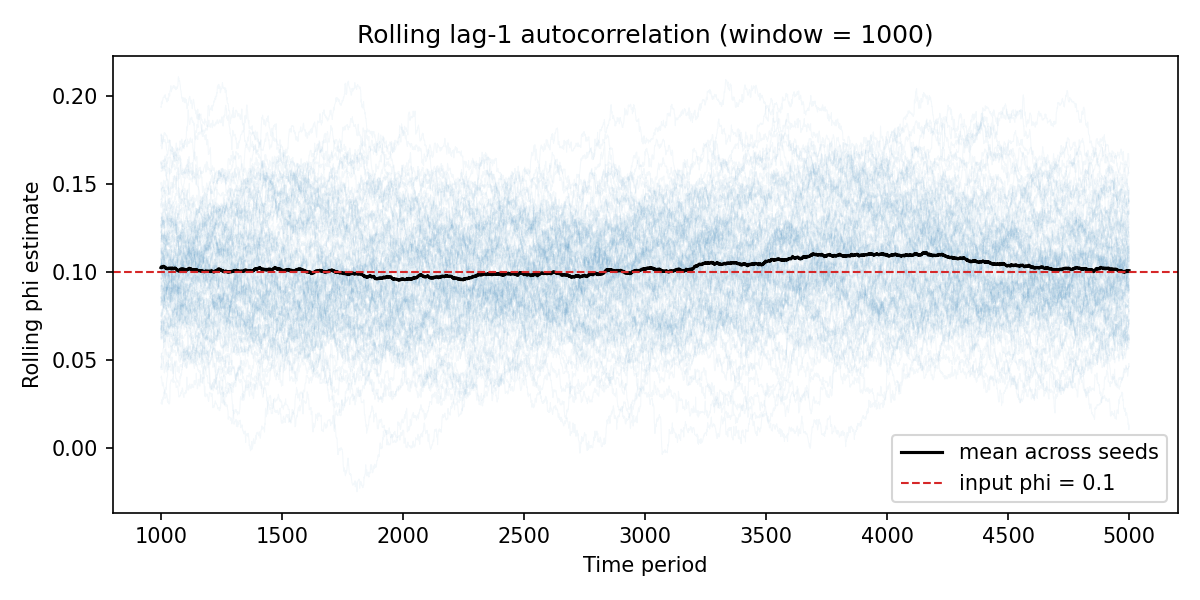
\includegraphics[width=0.78\textwidth]{../../results/figures/phase_02_rolling_phi.png}
\caption{Rolling lag-1 autocorrelation of returns under the null rule, estimated on a 1000-period sliding window for each of 100 seeds (faint lines). The black line is the cross-seed mean and the dashed line marks the input $\varphi=0.10$. The mean trace stays flat for the full run, with a total range of $0.016$ over the 4001 periods where the window is complete, so the effective AR coefficient shows no drift in the absence of adoption.} % src: phase_02_benchmark.npz['mean_phi_trace'], ['rolling_window'], ['seeds']
\label{fig:phase02-rolling-phi}
\end{figure}

% appendix B candidate: phase_01_return_histogram.png

\subsection{AR forecast performance without adoption (phase 3)}

Phase 3 attaches the rolling AR(1) forecasting rule of section 3.4 of the proposal to the null-market design of the previous subsection, in offline mode: the forecast is estimated and scored, but no trader acts on it. A single run uses $N=200$ traders, $T=8000$ periods, $\mu=0.05$, $\sigma=0.01$, $\sigma_q=1.0$, and seed 43, with the input autoregressive coefficient raised to $\varphi=0.25$ so the rule has a clearly detectable signal to recover. % src: notebooks/phase_03_ar_forecast.ipynb parameters cell (cell 1); phase_03_ar_forecast.npz['phi_input'], ['seed']
Each period the rule fits an AR(1) by least squares on the most recent $w \in \{50, 100, 250\}$ returns and issues a strictly out-of-sample one-step forecast $\hat{r}^{(A)}_{t+1}$, scored post hoc against realised returns by out-of-sample $R^{2}$ against a constant-mean benchmark (section 4.1 of the proposal), tracked on a trailing 1000-period window, and by full-sample mean squared forecast error (MSFE). % src: phase_03_ar_forecast.npz['ar_windows'], ['ar_order'], ['eval_window']; src/reflexive_market/metrics.py rolling_oos_r2(), msfe()
With zero adoption the realised return and the demand-adjusted return $x_{t+1} = r_{t+1} - \mu D_t$ differ only by unpredictable null-order impact, so this subsection reports realised-return performance only; the two targets separate once adopters start trading in phase 4. % src: notebooks/phase_03_ar_forecast.ipynb title cell (cell 0), note on realised vs demand-adjusted return

The rule recovers the signal it was built for. The mean rolling out-of-sample $R^{2}$ is small, positive for every window, and rising with window length: $0.013$ for $w=50$, $0.033$ for $w=100$, and $0.047$ for $w=250$. % src: phase_03_ar_forecast.npz['summary'][:, 2]
Figure~\ref{fig:phase03-rolling-oos-r2} shows the time profile: the traces co-move because they score one path, longer windows sit almost everywhere higher, and the share of periods with positive $R^{2}$ rises with $w$. The $w=250$ trace is positive at every evaluated period (minimum $0.020$), $w=100$ in $98.5$ percent of periods, while $w=50$ dips below zero in roughly $16$ percent. % src: rolling_oos_r2 traces recomputed from notebooks/phase_03_ar_forecast.ipynb parameters cell and seed 43 (reproduces npz summary exactly); w=50 sits below both longer windows at every common period, but w=100 exceeds w=250 in 68 of 6751 common periods (6781 to 6915, max gap 0.0047), hence "almost everywhere"; results/figures/phase_03_rolling_oos_r2.png
These levels are consistent with the return law's ceiling: an oracle knowing $\varphi$ exactly would attain a population $R^{2}$ of $\varphi^{2}=0.0625$, which the longer windows approach from below as estimation noise shrinks. % src: phase_03_ar_forecast.npz['phi_input'] = 0.25; ceiling = phi^2 follows from the return law (eq. 6 of the proposal) with iid null-order demand
The coefficient estimates tell the same story: the rolling $\hat{\varphi}$ fluctuates around the input value, with means $0.195$, $0.217$, and $0.229$ and standard deviations $0.145$, $0.103$, and $0.063$ for $w=50$, $100$, and $250$; the mild downward gap reflects the small-sample bias of least-squares AR(1) estimation together with single-path sampling noise, and closes as the window lengthens. % src: phase_03_ar_forecast.npz['summary'][:, 3] (means); stds recomputed from the notebook parameters cell and seed 43; results/figures/phase_03_ar_coefficients.png
Full-sample MSFE is nearly flat across windows ($1.18\times10^{-4}$ to $1.15\times10^{-4}$) and the rolling MSFE traces show no trend, as expected when no trader acts on the forecast. % src: phase_03_ar_forecast.npz['summary'][:, 1]; results/figures/phase_03_rolling_msfe.png
Sign accuracy, a diagnostic rather than an endpoint (section 4.2 of the proposal), is $0.56$ for the two shorter windows and $0.57$ for $w=250$. % src: phase_03_ar_forecast.npz['summary'][:, 4] (0.5592, 0.5592, 0.5732)

This completes the pre-adoption baseline. The previous subsection showed that the market does not drift when no one trades on a forecast; this one shows that the rolling rule recovers the linear-persistence signal at a known level, a small, stable, positive out-of-sample $R^{2}$ due entirely to the $\varphi r_t$ term.

\begin{figure}[h]
\centering
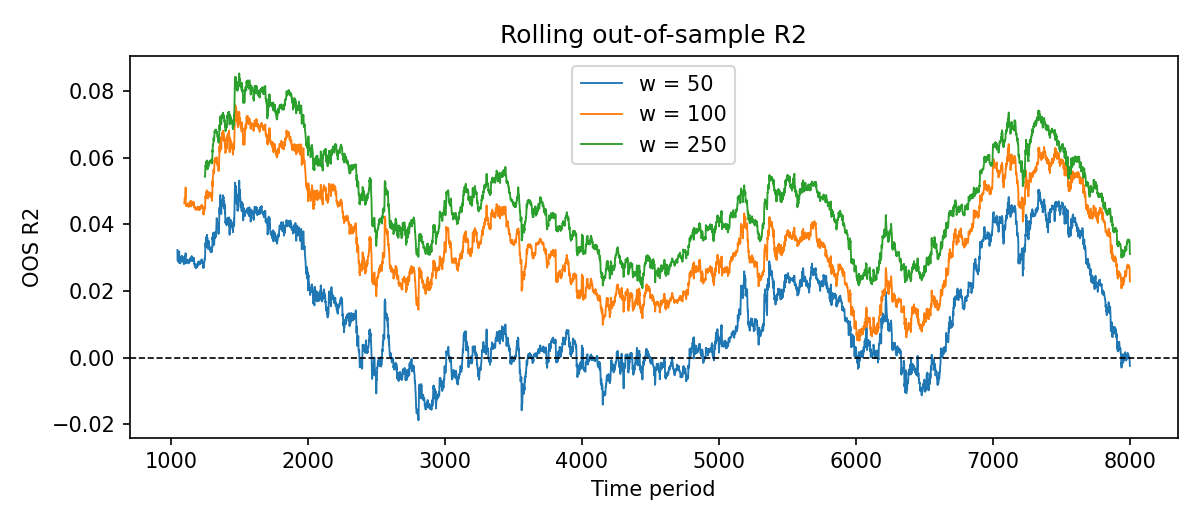
\includegraphics[width=0.78\textwidth]{../../results/figures/phase_03_rolling_oos_r2.png}
\caption{Rolling out-of-sample $R^{2}$ of the one-step AR(1) forecast against realised returns, computed on a trailing 1000-period window, for estimation windows $w=50$, $100$, and $250$ applied to the same null-market path (input $\varphi=0.25$, seed 43). The dashed line marks zero. The traces co-move because they score one path; longer windows sit almost everywhere higher (the $w=100$ and $w=250$ traces briefly cross around periods 6800 to 6900), the $w=250$ trace stays positive at every evaluated period, and the $w=50$ trace intermittently dips below zero.} % src: results/figures/phase_03_rolling_oos_r2.png; phase_03_ar_forecast.npz['eval_window'], ['phi_input'], ['seed']; sign and crossing statements recomputed from the notebook parameters cell and seed 43 (w=100 > w=250 in 68 of 6751 common periods, 6781 to 6915)
\label{fig:phase03-rolling-oos-r2}
\end{figure}

% appendix B candidate: phase_03_ar_coefficients.png

\subsection{Dual-channel result under stochastic adoption (phase 4)}

Phase 4 turns the offline forecast of the previous subsection into a tradeable rule and lets its use spread. Adopters map the shared rolling AR(1) forecast ($w=250$) into positions through the mean-variance demand of equation (1) of the proposal, clipped at the position cap of equation (3); non-adopters keep the random null rule. % src: notebooks/phase_04_stochastic_adoption.ipynb parameters cell (cell 1); phase_04_stochastic_adoption.npz['forecast_window']
With combined risk scaling $a\sigma^{2}=0.001$ and per-trader cap $\bar{q}=0.05$ the cap binds in nearly every period, so adopters are effectively fixed-size traders on the forecast's sign and their impact stays comparable in magnitude to the $\varphi r_t$ term rather than dominating it. % src: phase_04_stochastic_adoption.npz['risk_scale'], ['q_cap']; notebooks/phase_04_stochastic_adoption.ipynb cell 1 (comment on q_cap)
Adoption follows the stochastic diffusion of equations (12) and (13) of the proposal in three regimes: zero adoption ($\pi=0$), slow diffusion ($\pi=3\times10^{-4}$), and fast diffusion ($\pi=10^{-3}$), each with exit probability $\delta=0$, run on paired shocks from the shared seed 71 so that differences across regimes are attributable to adoption alone. % src: phase_04_stochastic_adoption.npz['regime_names'], ['regime_pi'], ['regime_delta'], ['seed']
The market is otherwise the phase 3 configuration ($N=200$, $T=8000$, $\mu=0.05$, input $\varphi=0.25$, $\sigma=0.01$, $\sigma_q=1.0$), with every rolling metric computed on a trailing 1000-period window. % src: phase_04_stochastic_adoption.npz['N'], ['T'], ['mu'], ['phi_input'], ['eval_window']; notebooks/phase_04_stochastic_adoption.ipynb cell 1 (sigma_news, sigma_q)
Adoption is held at zero until period 1250, the first period with a complete metric window, and the headline comparison contrasts a low-adoption window (periods 1250 to 2750) with a high-adoption window (the final 1500 periods), by which point the slow regime has reached a mean adoption share of 0.836 and the fast regime 0.994. % src: notebooks/phase_04_stochastic_adoption.ipynb cells 1 and 4 (adoption_start_t = 1250, summary_span = 1500); phase_04_stochastic_adoption.npz['summary'][:, 1]

Against realised returns, the forecast improves as adoption rises. In the high-adoption window the fast regime's rolling out-of-sample $R^{2}$ against $r_{t+1}$ is 0.190, versus 0.070 for the zero-adoption control on the same shocks (0.065 in the control's own late window), with the slow regime in between at 0.165. % src: phase_04_stochastic_adoption.npz['summary'][2, 3] = 0.1904, [0, 2] = 0.0695, [0, 3] = 0.0653, [1, 3] = 0.1651
The control row is the right low-adoption anchor: diffusion at $\pi=10^{-3}$ is fast enough that the fast regime's own early window already averages an adoption share of 0.505, with realised $R^{2}$ already lifted to 0.094. % src: phase_04_stochastic_adoption.npz['summary'][2, 0] = 0.5048, [2, 2] = 0.0942
The mechanism is the decomposition $r_{t+1}=\mu D_t + x_{t+1}$ of equation (7) of the proposal: every adopter trades in the direction of the same public forecast, so coordinated adopter demand pushes the realised return in the forecast direction, and the forecast scores partly against its own price impact. The left panel of Figure~\ref{fig:phase04-oos-r2-vs-adoption} shows that this is not a one-seed accident: pooled across 100 Monte Carlo seeds, the mean realised-return $R^{2}$ rises monotonically in adoption share. % src: notebooks/phase_04_stochastic_adoption.ipynb cells 21 and 23 (num_seeds_mc = 100, mc_base_seed = 1000); results/figures/phase_04_oos_r2_vs_adoption_mc.png

The same forecast on the same path is simultaneously losing the signal it was built to exploit. Scored against the demand-adjusted return $x_{t+1}=r_{t+1}-\mu D_t$, the counterfactual that strips out the contemporaneous demand impact while leaving the lagged-return component $\varphi r_t$ and the news shock in place (it is not the full regression residual; section 3.6 of the proposal), the rolling out-of-sample $R^{2}$ falls to 0.039 in the fast regime's high-adoption window, versus 0.082 under the control, with the slow regime at 0.047. % src: phase_04_stochastic_adoption.npz['summary'][2, 5] = 0.0386, [0, 4] = 0.0821, [1, 5] = 0.0471; definition per proposal sections 3.1.5 and 3.6 (eq. 7)
This reading asks whether the forecast still carries independent predictive content once self-fulfilment is removed, and the answer weakens as adoption rises: in the right panel of Figure~\ref{fig:phase04-oos-r2-vs-adoption} the Monte Carlo mean declines as adoption rises, with the drop steepening at high adoption shares. % src: results/figures/phase_04_oos_r2_vs_adoption_mc.png

The rolling effective AR coefficient is the mechanical link between the two readings. Estimated as the lag-1 autocorrelation of realised returns on the same trailing window, it rises from 0.282 under the control, close to the input $\varphi=0.25$, to 0.447 in the fast regime's high-adoption window (Figure~\ref{fig:phase04-phi-vs-adoption}). % src: phase_04_stochastic_adoption.npz['summary'][0, 6] = 0.2821, [2, 7] = 0.4470, ['phi_input'] = 0.25
Adopter demand responds positively to recent returns through the forecast, so the impact term $\mu D_t$ reinforces the lagged-return component and measured persistence grows with adoption. The rolling AR fit estimates its coefficient from realised returns, absorbs this amplified effective coefficient, and therefore systematically over-predicts the demand-adjusted process, whose own AR coefficient stays at the input 0.25 by construction; that over-prediction is the demand-adjusted decline of the previous paragraph. % src: mechanism per proposal section 4.1.3 (effective AR coefficient diagnostic); notebooks/phase_04_stochastic_adoption.ipynb cell 16 (markdown)
The control, meanwhile, moves far less across the same two windows (realised 0.070 to 0.065, demand-adjusted 0.082 to 0.068, effective coefficient 0.282 to 0.278), so the movements in the diffusion regimes are adoption effects, not time effects. % src: phase_04_stochastic_adoption.npz['summary'][0, :] = (0, 0, 0.0695, 0.0653, 0.0821, 0.0676, 0.2821, 0.2776)

This is the dual-channel result, and it is the headline finding of the report: adoption raises realised-return predictive performance through the self-fulfilment channel while eroding the independent demand-adjusted signal, on the same path and from the same forecast. Which reading a forecaster sees depends entirely on whether the evaluation target includes the forecaster's own price impact.

\begin{figure}[h]
\centering
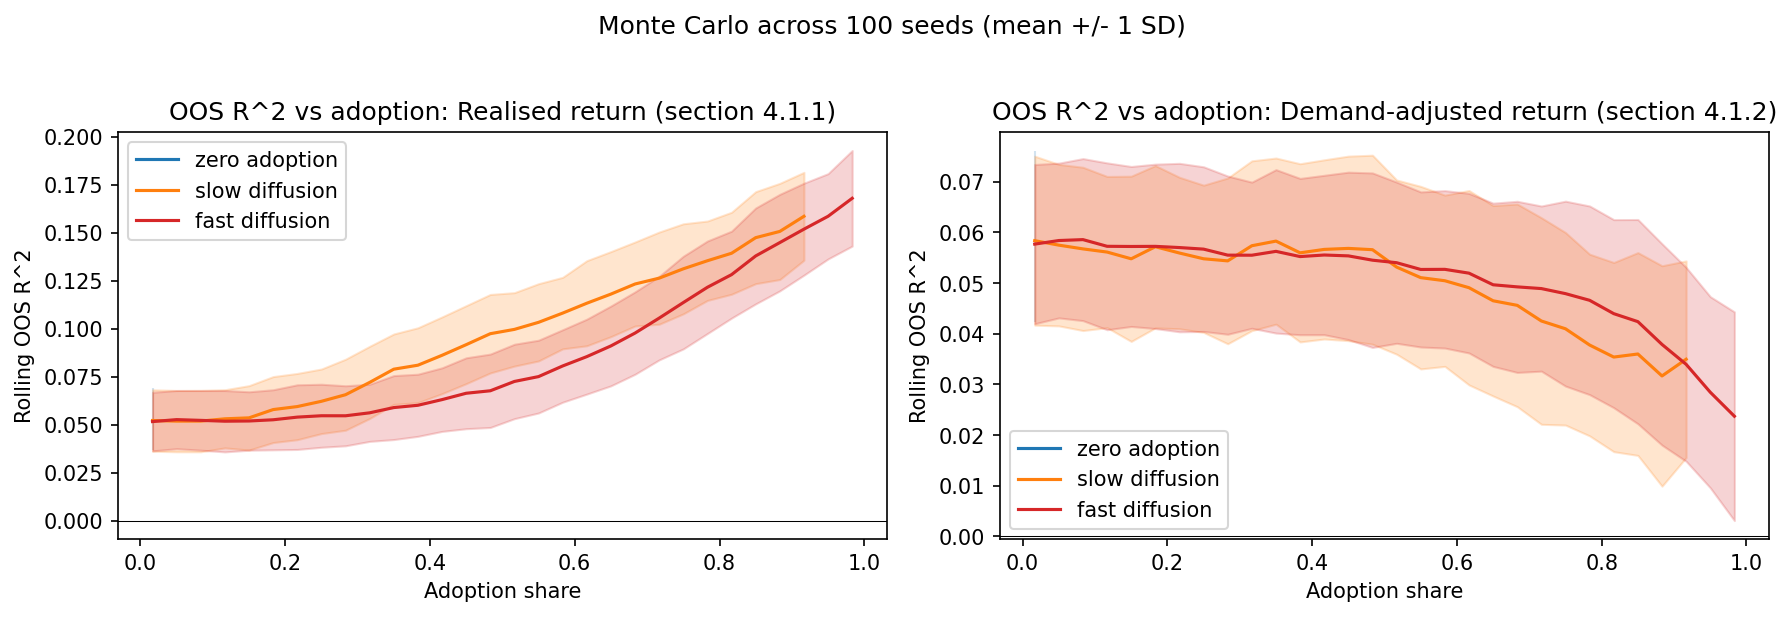
\includegraphics[width=0.78\textwidth]{../../results/figures/phase_04_oos_r2_vs_adoption_mc.png}
\caption{Rolling out-of-sample $R^{2}$ of the shared AR(1) forecast versus adoption share, pooled across 100 Monte Carlo seeds. The left panel scores the forecast against the realised return $r_{t+1}$ (self-fulfilling channel); the right panel scores the same forecast against the demand-adjusted return $x_{t+1}=r_{t+1}-\mu D_t$ (demand-adjusted-erosion channel); note the different y-axis scales. Lines are means within 30 adoption-share bins, pooling post-warm-up periods across seeds; shaded bands are $\pm 1$ standard deviation; bins with 10 or fewer observations are dropped, which trims the slow regime's curves short of full adoption. The zero-adoption regime contributes observations only at adoption share zero, a single bin, so it appears in the legend but draws no visible curve. The mean realised-return $R^{2}$ rises from about 0.05 near zero adoption to about 0.17 at full adoption, while the mean demand-adjusted $R^{2}$ falls from about 0.06 to about 0.02. The slow-diffusion curves sit slightly to the left of the fast curves because the trailing 1000-period metrics lag the instantaneous adoption share on the x axis, and the lag matters more the faster adoption ramps.} % src: results/figures/phase_04_oos_r2_vs_adoption_mc.png (endpoint values read from the rendered axes); notebooks/phase_04_stochastic_adoption.ipynb cells 20 to 23 (binning, band, drop rule, lag caveat); cell 21 output (slow regime max observed A = 0.925)
\label{fig:phase04-oos-r2-vs-adoption}
\end{figure}

\begin{figure}[h]
\centering
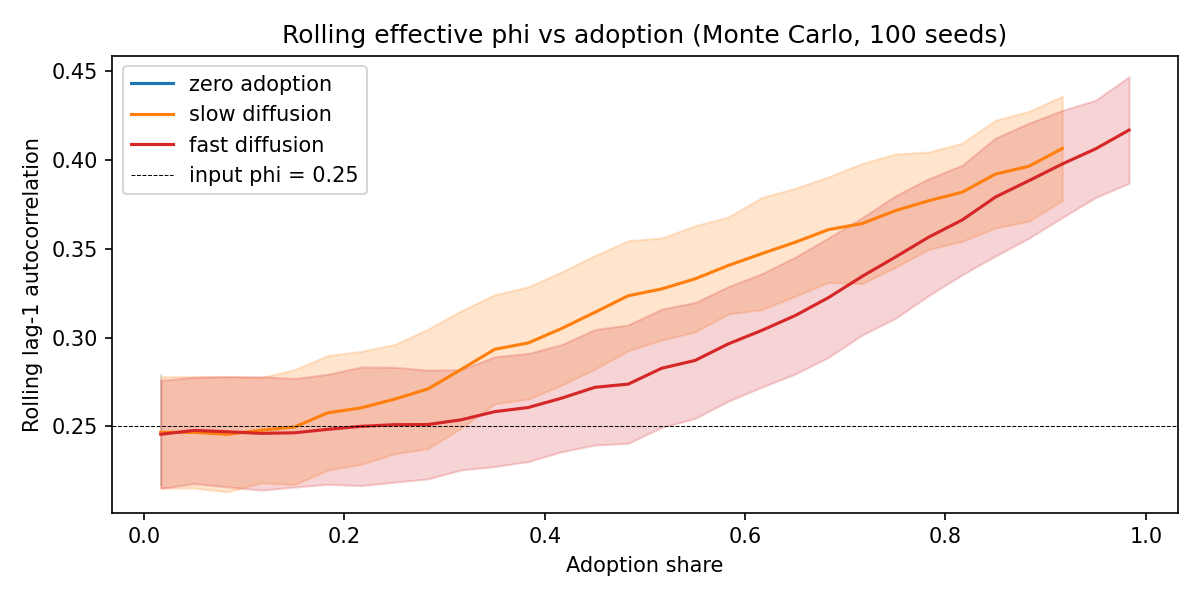
\includegraphics[width=0.78\textwidth]{../../results/figures/phase_04_phi_vs_adoption_mc.png}
\caption{Rolling lag-1 autocorrelation of realised returns versus adoption share, same Monte Carlo design as Figure~\ref{fig:phase04-oos-r2-vs-adoption} (100 seeds, 30 adoption-share bins, mean $\pm 1$ standard deviation, bins with 10 or fewer observations dropped). The dashed line marks the input $\varphi=0.25$. Both diffusion regimes start close to the input value near zero adoption and rise steadily with adoption share, reaching roughly 0.40 to 0.42 at their highest observed adoption shares; the zero-adoption regime occupies a single bin and draws no visible curve.} % src: results/figures/phase_04_phi_vs_adoption_mc.png (endpoint values read from the rendered axes); notebooks/phase_04_stochastic_adoption.ipynb cells 21 and 25
\label{fig:phase04-phi-vs-adoption}
\end{figure}

% appendix B candidate: phase_04_oos_r2_over_time.png

\subsection{Endogenous CE-based switching (phase 5)}

Phase 5 makes adoption respond to how the forecast is actually paying: the stochastic diffusion of equations (12) and (13) of the proposal is replaced by the risk-adjusted performance-based switching of its section 3.5. Each period the simulator records the realised one-period profit of equation (8) for a representative trader under each rule: the common capped adopter position, and a representative non-adopter's order. % src: notebooks/phase_05_performance_adoption.ipynb cell 0; src/reflexive_market/simulate.py run() docstring (null_profit, advanced_profit, eq. 8)
Each rule's certainty equivalent $\mathrm{CE}^{(k)}_t=\bar{\Pi}^{(k)}_t-\tfrac{a}{2}\,\hat{\sigma}^{2,(k)}_t$, the rolling mean profit net of a risk penalty on its rolling variance, is computed over $W_A=500$ periods with $a=1$, per equation (14), and each non-adopter switches to the advanced rule with the logistic probability $\Lambda(\alpha+\beta S_t)$ of equation (15) in the score gap $S_t=\mathrm{CE}^{(A)}_t-\mathrm{CE}^{(0)}_t$, with $\alpha=-5$ and $\beta=10000$. % src: phase_05_performance_adoption.npz['switching_window'] = 500, ['switching_a'] = 1.0, ['switching_alpha'] = -5.0, ['switching_beta'] = 10000.0; proposal section 3.5, eqs. (14) and (15)
At a zero score the implied switch probability is $\Lambda(-5)\approx0.0067$ per period, and score movements of order $10^{-4}$ move it strongly in either direction. % src: computed from phase_05_performance_adoption.npz['switching_alpha'] and ['switching_beta']: 1/(1+e^5) = 0.00669; beta = 1e4 makes a score of 1e-4 worth one logit
Everything else stays at the phase 4 configuration with adoption starting at period 1250; the comparator is the fast stochastic regime ($\pi=10^{-3}$) rerun on paired shocks from the shared seed 71, so any difference is attributable to the adoption mechanism. % src: phase_05_performance_adoption.npz['stochastic_pi'] = 1e-3, ['seed'] = 71, ['T'], ['N'], ['mu'], ['phi_input'], ['eval_window']; notebooks/phase_05_performance_adoption.ipynb cell 1 (adoption_start_t = 1250)

The adoption path changes shape; the erosion does not. The endogenous share is steplike. Through most of the run-up the score hovers slightly below zero (negative in 88 percent of pre-saturation periods, held down in part by the null rule's positive own-impact profit mean $\mu\sigma_q^{2}/N=2.5\times10^{-4}$), and at the median pre-saturation score the implied switch rate is 0.00049 per period, about half the comparator's diffusion rate, so the share mostly creeps; episodes of positive score raise the per-period inflow by a factor of about 3.6, producing the bursts. % src: recomputed from notebooks/phase_05_performance_adoption.ipynb parameters cell with seed 71 (deterministic rerun reproduces npz['summary'] exactly); all stats over the pre-saturation window t in [1250, 2842): S_t < 0 in 1397 of 1592 periods; median S = -2.61e-4, Lambda(-5 + 1e4 * (-2.61e-4)) = 0.00049, vs stochastic_pi = 1e-3; mean per-period share gain 0.00172 (S > 0) vs 0.00048 (S <= 0), consistent with the implied rate; E[null profit] = mu*sigma_q^2/N = 0.05*1.0/200 = 2.5e-4 per src/reflexive_market/simulate.py run() docstring
The endogenous run reaches full adoption by period 2842, while the stochastic share crosses 0.99 only at period 6164. % src: same rerun (first A = 1 at t = 2842; stochastic first A >= 0.99 at t = 6164); results/figures/phase_05_adoption_share.png
Yet over the same low- and high-adoption windows as the previous subsection the two regimes give nearly identical erosion readings: the demand-adjusted out-of-sample $R^{2}$ falls from 0.071 to 0.039 under stochastic diffusion and from 0.076 to 0.037 under performance switching, while the rolling effective AR coefficient rises from 0.320 to 0.447 and from 0.315 to 0.449 respectively, at mean adoption shares of 0.505 to 0.994 and 0.455 to 1.000. % src: phase_05_performance_adoption.npz['summary'] (rows: stochastic diffusion, performance switching; cols: A_low, A_high, R2da_low, R2da_high, phi_low, phi_high)
Figure~\ref{fig:phase05-erosion-vs-adoption} traces both diagnostics against the adoption share itself: the two regimes start from the same pre-adoption values, decline and rise along overlapping paths, and converge at full adoption. % src: results/figures/phase_05_erosion_vs_adoption.png; rerun: first finite rolling demand-adjusted R^2 = 0.1041 at t = 1249 (identical across regimes pre-adoption)
The performance-switching curve sits somewhat above the stochastic one on the demand-adjusted panel at intermediate shares; this is a lag artefact: the endogenous run sweeps those shares too quickly for the trailing 1000-period metric window to refresh (235 periods between shares 0.6 and 0.95, against 1945 for the diffusion run). % src: rerun: 235 periods with A in [0.6, 0.95] (performance switching) vs 1945 (stochastic diffusion); results/figures/phase_05_erosion_vs_adoption.png left panel

Endogenous switching therefore changes when the market visits each adoption level, not what adoption does once there: at matched shares both mechanisms produce the same demand-adjusted decline and the same effective-coefficient amplification. The dual-channel result of the previous subsection is thus not an artefact of the exogenous diffusion assumption; erosion is a property of the adoption share, however the share is generated. The run also shows why the mechanism reinforces rather than brakes adoption in the cost-free baseline: adopter trades strengthen the autoregressive component of realised returns, so the advanced rule's certainty equivalent pulls level and then ahead as adoption builds (the score's pre-saturation maximum arrives one period before full adoption), and nothing pushes the score decisively negative at high adoption. % src: rerun: max pre-saturation S_t = +3.0e-4 at t = 2841, one period before first A = 1 at t = 2842; results/figures/phase_05_switching_score.png (the larger spike to +0.0064 occurs after full adoption)
Whether transaction costs change that is taken up in section~\ref{sec:phase7-results}.

\begin{figure}[h]
\centering
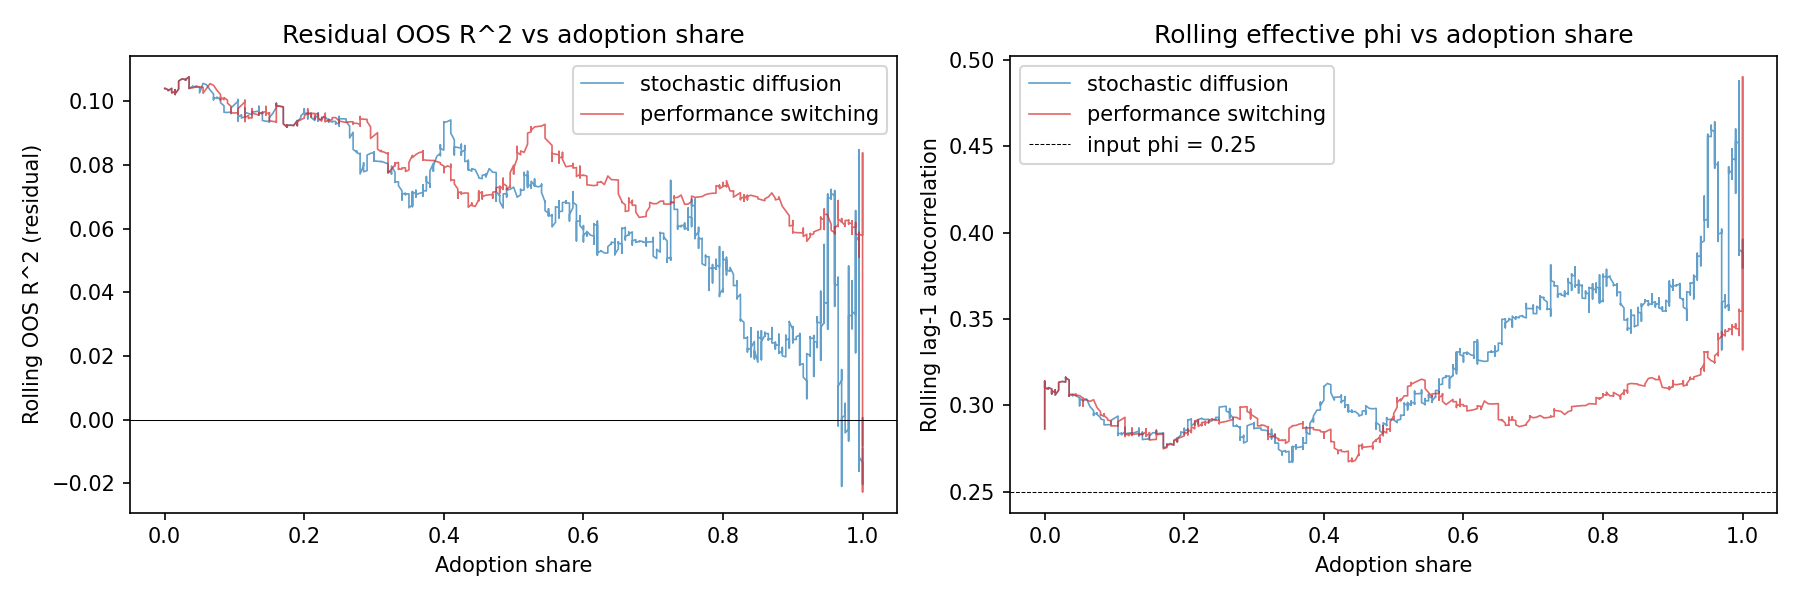
\includegraphics[width=0.78\textwidth]{../../results/figures/phase_05_erosion_vs_adoption.png}
\caption{Rolling out-of-sample $R^{2}$ against the demand-adjusted return (left) and rolling lag-1 autocorrelation of realised returns (right), plotted against the adoption share for exogenous stochastic diffusion ($\pi=10^{-3}$) and endogenous CE-based switching on the same paired shocks (seed 71); both metrics use a trailing 1000-period window. The two regimes share the pre-adoption segment (demand-adjusted $R^{2}$ near 0.104 and effective coefficient between 0.286 and 0.314 at zero adoption, against the input $\varphi=0.25$ marked by the dashed line), then decline (left) and rise (right) along overlapping paths as the share grows, converging at full adoption. The performance-switching curve sits above the stochastic one on the left panel at intermediate shares because the endogenous run sweeps those shares in few periods relative to the metric window; the vertical segments at share 1.0 collect each run's post-saturation stretch.} % src: results/figures/phase_05_erosion_vs_adoption.png; phase_05_performance_adoption.npz['stochastic_pi'], ['seed'], ['eval_window'], ['phi_input']; rerun: plotted effective phi at zero adoption spans 0.286 to 0.314, first finite demand-adjusted R^2 = 0.1041
\label{fig:phase05-erosion-vs-adoption}
\end{figure}

% appendix B candidate: phase_05_adoption_share.png
% appendix B candidate: phase_05_switching_score.png

\subsection{Parameter sweep and critical adoption shares (phase 6)}

\subsection{Transaction-cost extension and economic endpoint (phase 7)}\label{sec:phase7-results}


\section{Discussion}

\subsection{Interpretation of the dual-channel mechanism}

\subsection{Why the effective AR coefficient rises with adoption}

\subsection{Boundary conditions and the realised-channel non-result}

\subsection{Limitations}


\section{Conclusion}

\subsection{Summary of findings}

\subsection{Implications for forecasting under adoption}

\subsection{Directions for future work}


\bibliography{references}


\appendix

\section{Model equations and derivations}

\section{Additional figures}

\section{Parameter tables and reproducibility details}

\end{document}
